\documentclass{article}
\usepackage[paperwidth=960pt,paperheight=540pt,margin=32pt]{geometry}
\usepackage{fontspec,xeCJK,graphicx,xcolor,hyperref}
\setmainfont{TeX Gyre Heros}\setCJKmainfont{Noto Sans CJK SC}
\definecolor{ink}{HTML}{102B30}\definecolor{green}{HTML}{247D70}
\pagecolor{white}\color{ink}\pagestyle{empty}
\hypersetup{pdfauthor={AURORA Research Team},pdftitle={AURORA 界面与结果展示}}
\setlength{\parindent}{0pt}
\begin{document}
{\fontsize{27}{34}\selectfont\bfseries report 结果展示：条件候选与后续复核}\par\vspace{12pt}
\begin{center}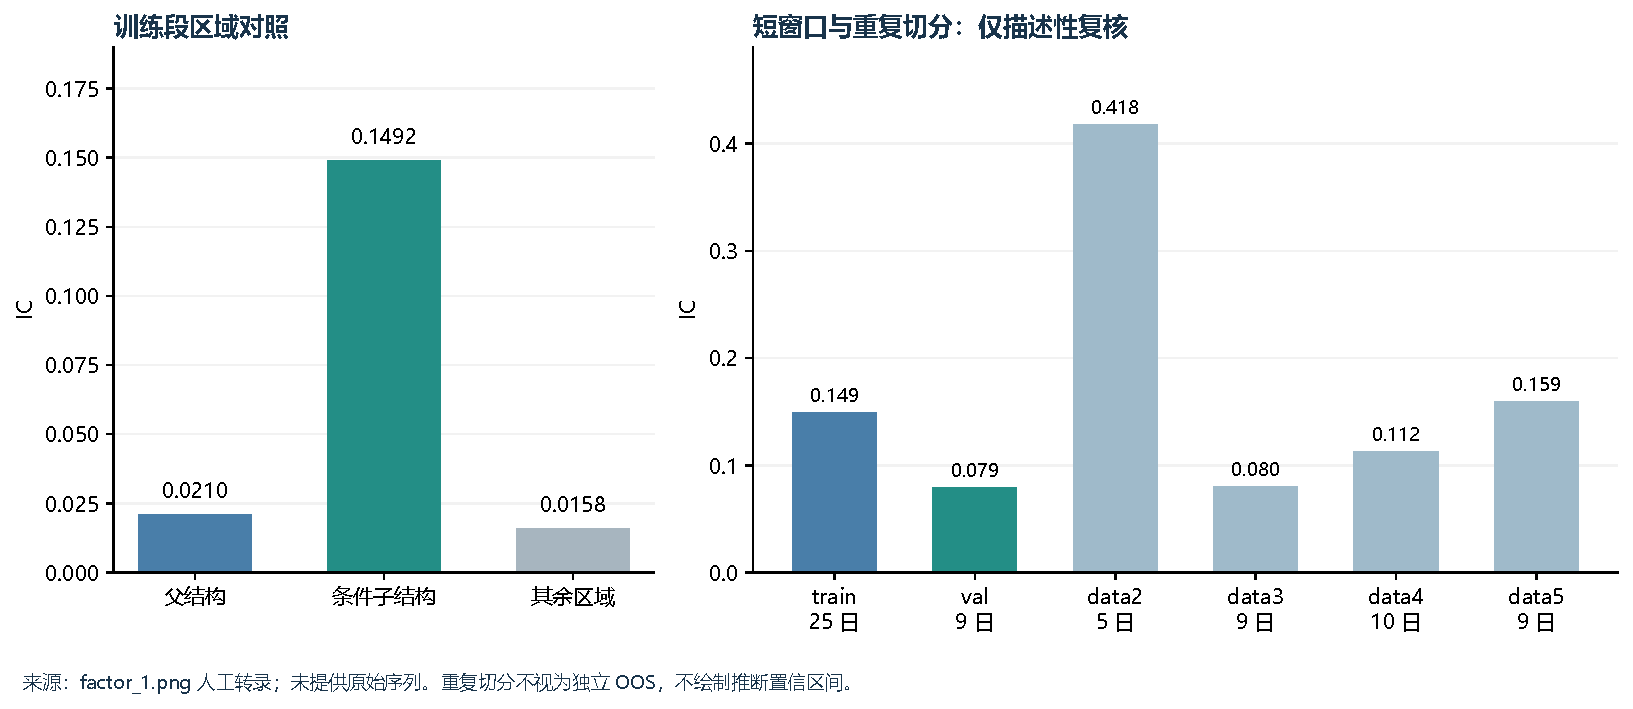
\includegraphics[width=890pt,height=365pt,keepaspectratio]{../figures/corelab_case.pdf}\end{center}
\vfill{\fontsize{14}{20}\selectfont 父 IC 0.0210；条件区域 IC 0.1492；验证 IC 0.0793，HAC t = 0.905，仅 9 日。}\par
\end{document}
